\status{review}
\chapter{BGO Calibrations}
\begin{refsection}
{\itshape The BGO is an auxiliary detector of the MEG II apparatus. It is usually used during the CEX calibration, as discussed in Ch.~\ref{ch:MEG:CEX}, but it was also part of the X17 data-taking discussed in Ch~\ref{ch:X17}. Here we will see how the calibration (and inter-calibration) is tackled. I worked on this item with a master student from ETH, David St\"{a}ger, who compiled all the information in his thesis \cite{David}.}
\label{ch:BGO}\\

\noindent
Calibrating a calorimeter involves establishing a relationship between the observed waveforms in the PMT readout channels and the energy of incoming photons. 
In the case of calibrating the BGO, we assume the energy deposited by the photon ($E_\g$) is directly proportional to the observed PMT charge ($I_j$) in each channel, considering that the energy can be distributed across multiple crystals (Eq.~\ref{eq:BGO}). 
The calibration factors ($f_j$) for each channel are determined from real data. 
However, since many detector processes are energy-dependent, the BGO response may not be strictly linear, especially away from the calibration point. To address this, calibration is done close to the 18.15 MeV transition of excited \ce{^8Be}, which is crucial for the X17 measurement. 
Hence, calibration is performed using the 17.64 MeV transition of \ce{^8Be}, excited by protons with a kinetic energy of 500 keV. 
Various collected datasets are available for calibration purposes, as listed in Tab.~\ref{tab:datasets}.

\begin{equation}
    E_\g = \sum_{j=0}^{15}I_j\cdot f_j
    \label{eq:BGO}
\end{equation}

    \begin{table}[h]
        \centering
        \begin{tabular}{|c|c|c|c|}
        \hline
        Date & Runs & $E_p$ [keV] & $I_{CW}$ [$\mu$A] \\
        \hline
        29.01.2023 & 482350 - 482425 & 500 & 2 \\
        30.01.2023 & 482539 - 482628 & 500 & 2 \\
        31.01.2023 & 482784 - 482828 & 500 & 3 \\
        28.02.2023 & 510122 - 510171 & 500 & 6 \\
        \hline
        \end{tabular}
        \caption{Collected datasets for the BGO calibration.}
    \label{tab:datasets}
    \end{table}

\status{review}
\section{Calibration factors}
    To calibrate the detector, we determine calibration factors $f_j$ for each of the 16 channels using photons emitted in the $\text{Li} + p \rightarrow \text{Be} + \gamma$ reaction at $E_p = \SI{500}{keV}$. 
    Since the reaction yields a continuous spectrum, due to the width of the 15.6 MeV line, we adjust the observed spectrum by shifting peaks to expected energies in a step procedure:
    \begin{outline}
        \1[1st] We introduce a scale factor $K_{scale}$ to relate the charge $I_j$ to the energy $$E'_j=K_{scale}\cdot I_j$$
        \1[2nd] We ensure uniform channel response by scaling each channel's spectrum by a factor $a_j$, determined by shifting peaks to \SI{17.64}{MeV}. $$E''_j=K_{scale} a_j \cdot I_j$$
        \1[3nd] We sum energy contributions of all channels, considering only events where the highest charge is in central crystals. We introduce $K_{leak}$ to shift the rightmost peak to \SI{17.64}{MeV}, accounting for energy leakage between crystals. The reconstructed energy deposit is: $$E_{\gamma} = \sum_{j=0}^{15} K_{\text{scale}} \cdot K_{\text{leak}} \cdot a_j \cdot I_j$$.
    \end{outline}
    
    \noindent
    The steps are highlighted in Fig.~\ref{fig:BGO:intercalibration} and Fig.~\ref{fig:BGO:leak}.
    For convenience, we split calibration factors into $f_j = K_{\text{scale}} \cdot K_{leak} \cdot a_j = K_{scale} \cdot c_j$, where $c_j$ is determined from data after selecting a $K_{\text{scale}}$.

    \begin{figure}[]
        \centering
        \subfloat[The single channels are fitted with a doublegauss to find the peak.]{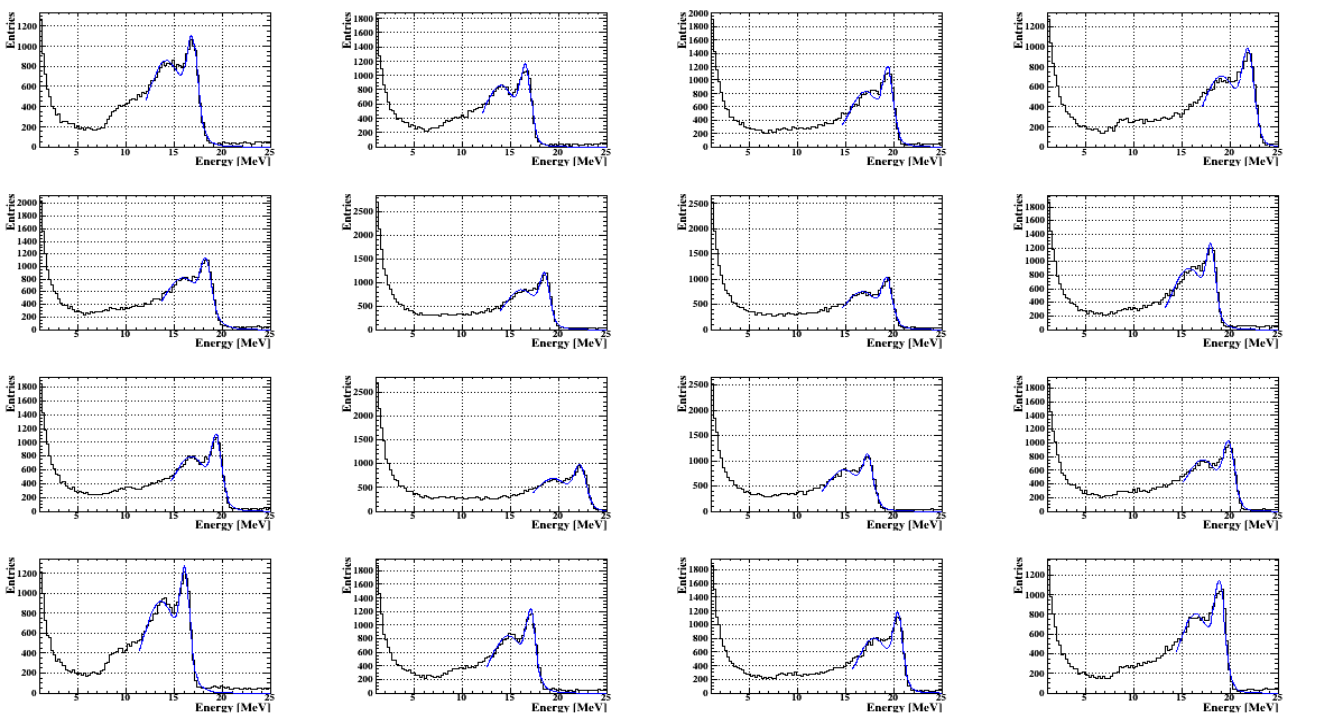
\includegraphics[width=0.9\textwidth]{Figures/X17/BGO/BGO_doublegauss.png}}\\
        \subfloat[Intercalibration factors $a_j$ are applied to alligne the peaks.]{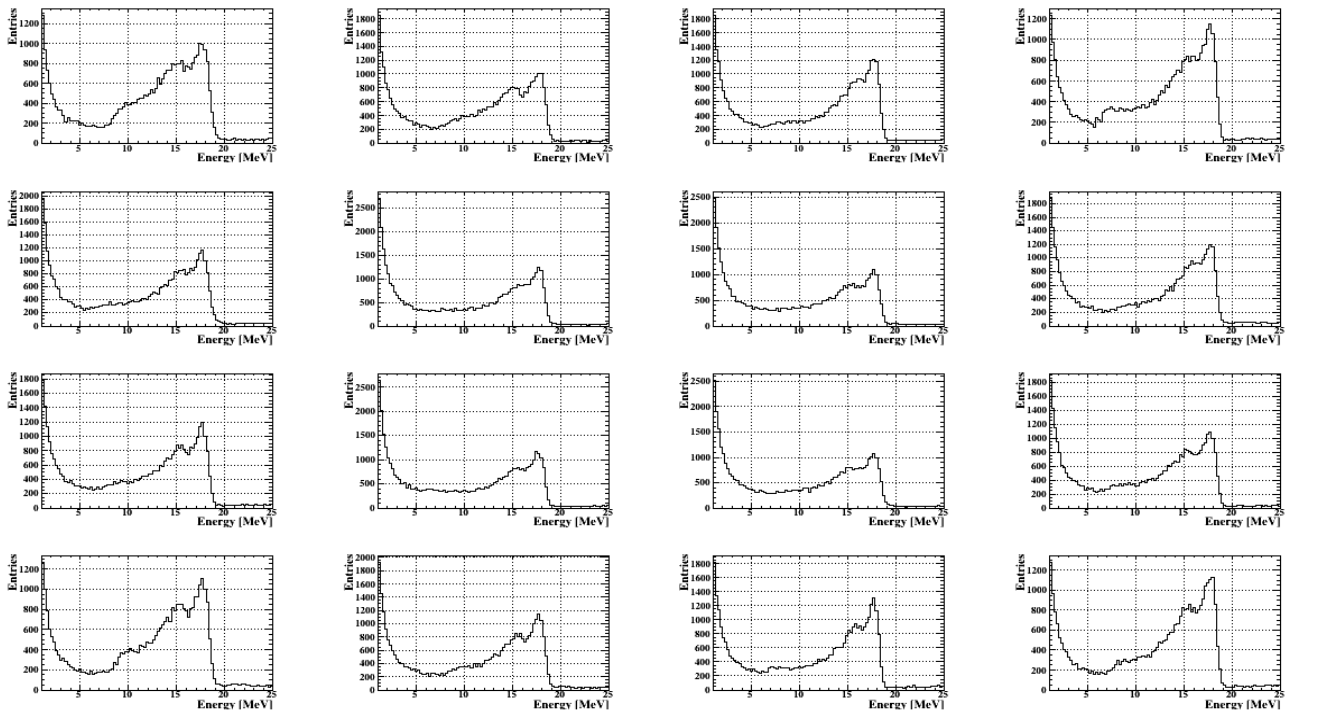
\includegraphics[width=0.9\textwidth]{Figures/X17/BGO/BGO_intercalibration.png}}
        \caption[BGO: intercalibration]{We start by fitting the single channel (multiplied by $K_{scale}$) to allign them.}
        \label{fig:BGO:intercalibration}
    \end{figure}

    \begin{figure}[]
        \centering
        \subfloat[The spectrum is the sum of the aligned channels.]{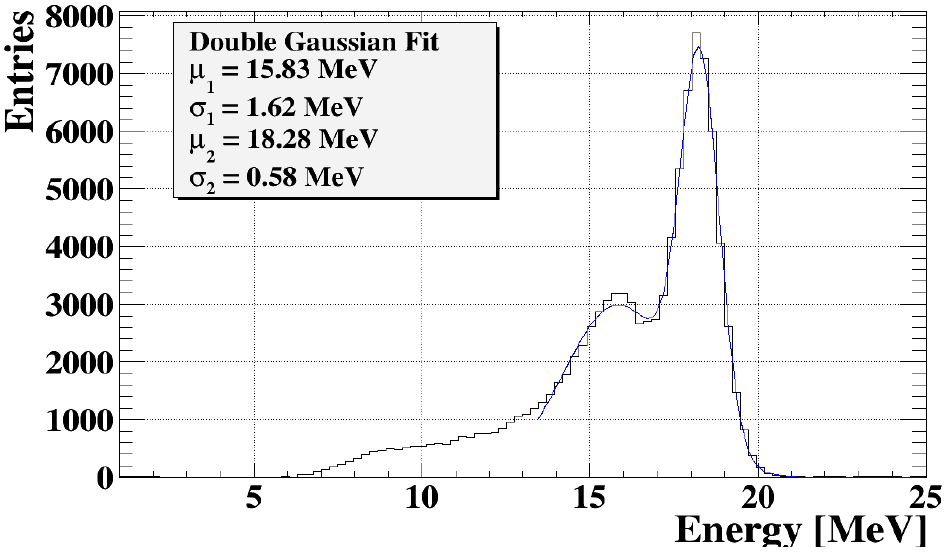
\includegraphics[height=4.5cm]{Figures/X17/BGO/BGO_noleak.png}}
        \subfloat[The spectrum needs to be corrected with $K_{leak}$.]{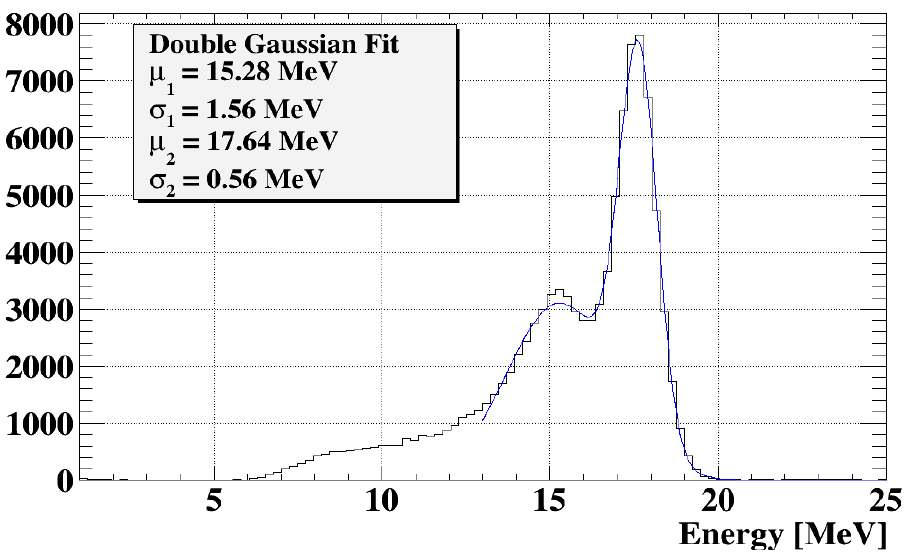
\includegraphics[height=4.5cm]{Figures/X17/BGO/BGO_leak.png}}
        \caption[BGO: introducing the leak]{The aligned channels sum is the BGO spectrum it is corrected for the leak between crystals.}
        \label{fig:BGO:leak}
    \end{figure}

    \status{review}
    \subsection{Sample size}
        To examine the sensitivity of calibration factors to sample size, we utilized a dataset of 90 runs collected on January 30, 2023, just before a month-long period of X17 data collection with no further calibration runs. 
        Initially, we determined calibration factors using the described procedure for the entire 90-run dataset.
        To assess variation with sample size, we created 500 sub-samples of N runs each, randomly selected from the full set. 
        For each subsample (with 50 and 30 runs, respectively), we computed the product of calibration factors $K_{leak} \cdot a_j$ and evaluated the mean and standard deviation. 
        The results, tabulated in Tab.~\ref{tab:calibration_factors} for N = 30 and N = 50, indicate the extent of variation in calibration factors with smaller sample sizes. 
        Notably, the mean calibration factor obtained from the 500 subsamples aligns with that from the full dataset. 
        Across tested sample sizes, the standard deviation of the product $K_{leak} \cdot a_j$ remained below 0.5\%.
        
        \begin{table}[h]
        \centering
        \begin{tabular}{|c|c|c|c|c|c|c|c|c|}
        \hline
        Channel & 0 & 1 & 2 & 3 & 4 & 5 & 6 & 7 \\
        \hline
        $c_j = K_{\text{leak}} \cdot a_j$ & 1.0106 & 1.0300 & 0.8793 & 0.7798 & 0.9311 & 0.9198 & 0.8845 & 0.9489 \\
        $\sigma_B$ (N = 30) & 0.0016 & 0.0019 & 0.0016 & 0.0013 & 0.0015 & 0.0012 & 0.0010 & 0.0016 \\
        $\sigma_B$ (N = 50) & 0.0010 & 0.0013 & 0.0011 & 0.0009 & 0.0010 & 0.0010 & 0.0007 & 0.0012 \\
        \hline
        \hline
        Channel & 8 & 9 & 10 & 11 & 12 & 13 & 14 & 15 \\
        \hline
        $c_j = K_{\text{leak}} \cdot a_j$ & 0.8799 & 0.7670 & 0.9858 & 0.8590 & 1.0593 & 0.9971 & 0.8357 & 0.9026 \\
        $\sigma_B$ (N = 30) & 0.0013 & 0.0010 & 0.0015 & 0.0015 & 0.0018 & 0.0014 & 0.0011 & 0.0020 \\
        $\sigma_B$ (N = 50) & 0.0009 & 0.0007 & 0.0010 & 0.0010 & 0.0011 & 0.0010 & 0.0007 & 0.0012 \\
        \hline
        \end{tabular}
        \caption{Calibration factors and standard deviations for different sample sizes.}
        \label{tab:calibration_factors}
        \end{table}

\status{review}
\section{Stability}
An interesting point is the time stability of the calibration. For this purpose, data were taken on three days: 29-30-31.01.2023. 
The variation, shown in Fig.~\ref{fig:BGO:stability:3days}, is found to be very dependent on the channel. 
This is not a problem because calibration runs were taken every day to follow the evolution of the detectors.
When looking at the variation over a longer time, beginning-end of the data-taking, we find a systematic drift, shown in Fig.~\ref{fig:BGO:stability:StartFinish}.
The drift might be explained by a slow drop in the PMT voltage supply and can be compensated by assuming a linear dependence with time.
The difference of the peak position before and after linear correction is shown in Fig.~\ref{fig:BGO:correction}.

\begin{figure}
    \centering
    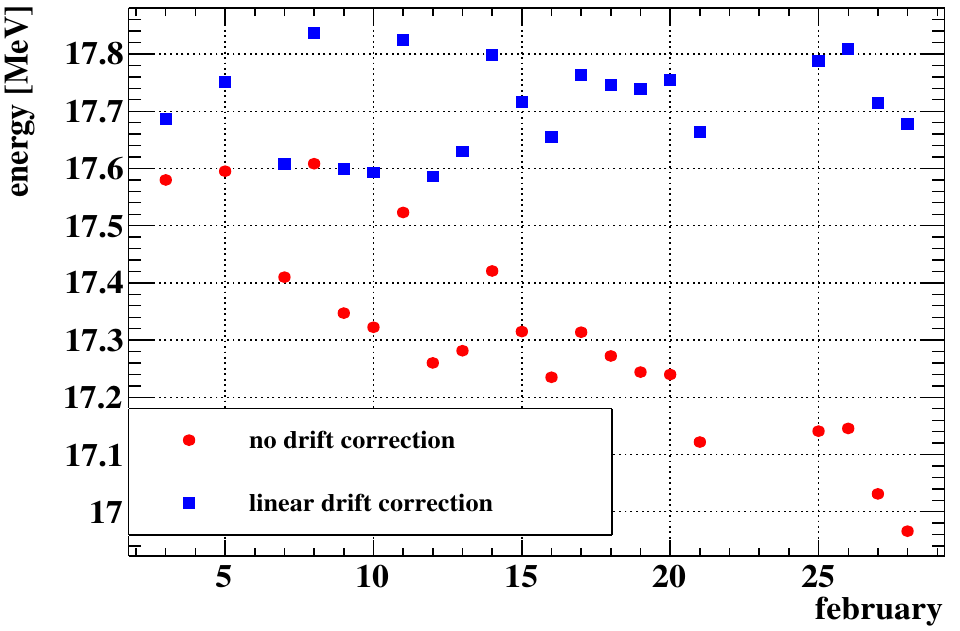
\includegraphics[width=0.9\linewidth]{Figures//X17//BGO/BGO_correction.png}
    \caption[BGO: linear correction to the 17.6 MeV line]{History of the 17.6 MeV line with and without linear correction for the drift found in Fig.~\ref{fig:BGO:stability:StartFinish}.}
    \label{fig:BGO:correction}
\end{figure}

\begin{figure}
    \centering
    \subfloat[The change of the calibration factors on 3 days span.]{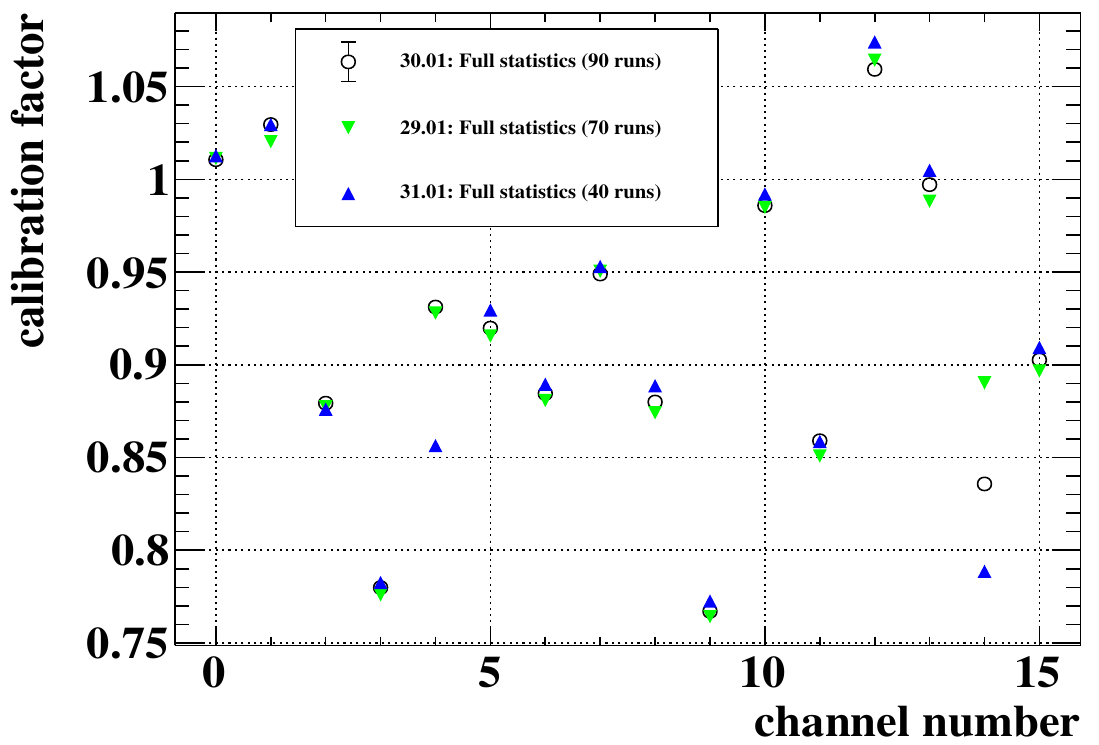
\includegraphics[width=0.9\textwidth]{Figures/X17/BGO/BGO_calibration_3days.png}\label{fig:BGO:stability:3days}}\\
    \subfloat[Drift of the calibration factors between start and finish of the data-taking period (29 days).]{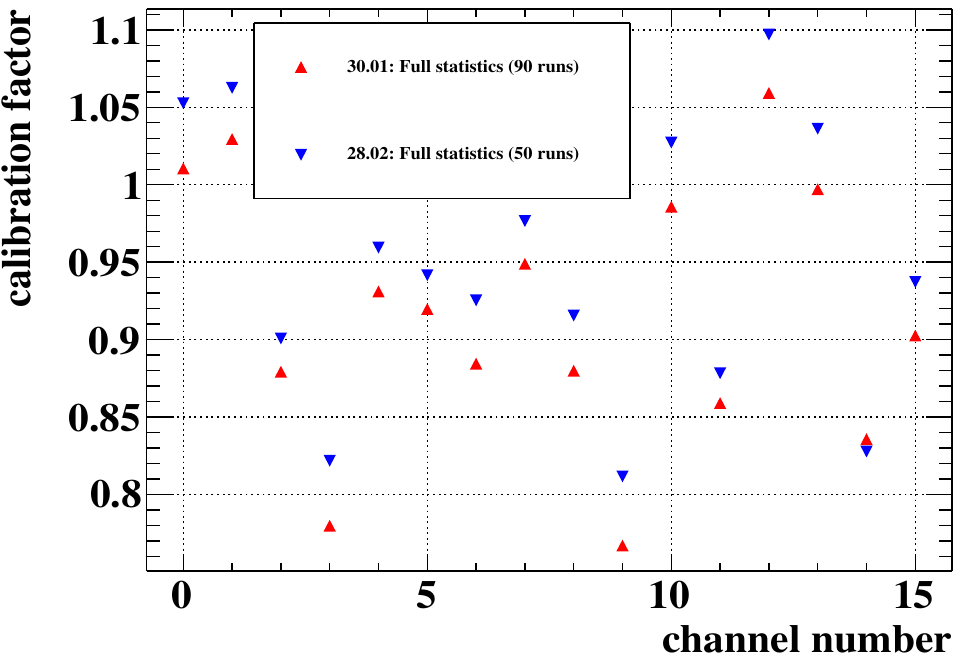
\includegraphics[width=0.9\textwidth]{Figures/X17/BGO/BGO_calibration_StartStop.png}\label{fig:BGO:stability:StartFinish}}   
    \caption{Time stability of the calibration factors: (a) 3 days, (b) start and finish of the data-taking.}
\end{figure}
\status{review}
\section*{Bibliography}
\printbibliography[heading=none]
\end{refsection}